\documentclass{article}

% if you need to pass options to natbib, use, e.g.:
%     \PassOptionsToPackage{numbers, compress}{natbib}
% before loading neurips_2019

% ready for submission
% \usepackage{neurips_2019}

% to compile a preprint version, e.g., for submission to arXiv, add add the
% [preprint] option:
%     \usepackage[preprint]{neurips_2019}

% to compile a camera-ready version, add the [final] option, e.g.:
     \usepackage[final]{neurips_2019}

\usepackage{amsmath}
\usepackage{algorithm}
\usepackage[noend]{algpseudocode}
% \usepackage[superscript,biblabel]{cite}

\usepackage[pdftex]{graphicx}
% to avoid loading the natbib package, add option nonatbib:
%     \usepackage[nonatbib]{neurips_2019}

\usepackage[utf8]{inputenc} % allow utf-8 input
\usepackage[T1]{fontenc}    % use 8-bit T1 fonts
\usepackage{hyperref}       % hyperlinks
\usepackage{url}            % simple URL typesetting
\usepackage{booktabs}       % professional-quality tables
\usepackage{amsfonts}       % blackboard math symbols
\usepackage{nicefrac}       % compact symbols for 1/2, etc.
\usepackage{microtype}      % microtypography

\title{A crossover code for high-dimensional composition}

% The \author macro works with any number of authors. There are two commands
% used to separate the names and addresses of multiple authors: \And and \AND.
%
% Using \And between authors leaves it to LaTeX to determine where to break the
% lines. Using \AND forces a line break at that point. So, if LaTeX puts 3 of 4
% authors names on the first line, and the last on the second line, try using
% \AND instead of \And before the third author name.

\author{%
  Rich Pang\\
  Computational Neuroscience Center\\
  University of Washington\\
  Seattle, WA 98195\\
  \texttt{rpang at uw dot edu} \\
  % examples of more authors
  % \And
  % Coauthor \\
  % Affiliation \\
  % Address \\
  % \texttt{email} \\
  % \AND
  % Coauthor \\
  % Affiliation \\
  % Address \\
  % \texttt{email} \\
  % \And
  % Coauthor \\
  % Affiliation \\
  % Address \\
  % \texttt{email} \\
  % \And
  % Coauthor \\
  % Affiliation \\
  % Address \\
  % \texttt{email} \\
}

\begin{document}

\maketitle

\begin{abstract}
We present a novel method for encoding compositional information by recursively weaving together high-dimensional (HD) random vectors. Inspired by chromosomal crossover, a fraction of one vector's components are masked out and replaced by those from another, via a context-dependent mask. Contrasting most HD computing schemes, "crossover" codes highly overlap with their base elements' and sub-structures' codes yet without sacrificing relational information, allowing fast element readout and decoding by greedy reconstruction. Crossover is mathematically tractable and has several properties desirable for robust, flexible representation.
\end{abstract}

\section{Introduction}

A common problem faced by intelligent systems is how to encode objects of variable complexity in fixed dimensions. Ideally, similar objects should have similar codes, new objects should not require rearranging existing codes, and there should be no limit on object complexity. Distributing codes across high-dimensional (HD) vectors yields robustness and potential flexibility and generalization \cite{Hinton:1984, Mikolov:2013}, but how does one store compositional relations, like order or binding in such a code, e.g. to distinguish AB vs BA or ((A,B), (C,D)) vs ((A,D), (C,B)), respectively? While trained networks have some implicit capacity for this \cite{Bahdanau:2014, Luong:2015, Wu:2016}, it is unclear (1) how such networks might encode complexity beyond that of their training data, and (2) how to quantify internal network representations \cite{Lipton:2016}. An alternative approach, known as HD computing (HDC), is to assign \textit{random} vector codes to a set of "base" elements of the data (e.g. symbols), and rules for composing these into richer data structures (e.g. words) \cite{Plate:1995, Kanerva:2009, Gayler:2004}. HDC's advantages are (1) random HD vectors have low overlap with high probability, enabling large element codebooks, (2) there is no hard limit on data complexity, and (3) encoding is often analytically tractable. While most systems would of course require some training on environment statistics, HDC provides a compelling blueprint for representational flexibility.

Most HDC schemes use codes in which relations among elements can be easily recovered, but only if one provides certain elements as cues (e.g. cue A recovers B from ((A,B),(C,D))). Typical relation-encoding operations include circular convolution \cite{Plate:1995}, permutation \cite{Gayler:1998, Sahlgren:2008}, or matrix multiplication \cite{Gosmann:2019}, which create relational codes that little overlap their elements' codes (e.g. AB's code is distinct from A's and B's). This low overlap means elements cannot be directly recovered from the relation code (although see \cite{Rachkovskij:2001}), and it conflicts with our desire that AB should resemble A and B more than C. Here, we present a new way (to our knowledge) to encode compositional relations, where two HD vectors $X$ and $X'$ are ordered or bound by masking out a fraction of $X$'s components and replacing them with those from $X'$, analogous to chromosomal crossover, and with relational information encoded in the context-dependent mask $\mu(X, X')$. As a result, "crossover" composition codes highly overlap with the substructures and elements used to build them, allowing direct recovery of base elements and decoding by greedy reconstruction. Further, they distribute information evenly across components and have marginal statistics invariant to object complexity, suggesting utility for robust intelligent systems. We describe crossover for sequences first, then generalize to binding and trees.

\section{Results}

Let $X$ be a vector of $N$ components, each of which can take any of $Z$ states, $x_j \in G \equiv \{1,...,Z\}$, and let $d(X, X')$ be the Hamming distance from $X$ to $X'$. For a symbol sequence $Y = (y_1, ..., y_L)$, where $y_t \in D \equiv \{1, ..., M\}$, we establish a mapping from $Y$ to $X^Y$ as follows:

First sample a codebook $C \equiv \{X^1, ..., X^M, X^*\}$, where $X^*$ is a "start code", and $x^j$ are i.i.d. across all components and codes and sampled uniformly from $G$. Next sample a mask function $\mu$, an $N \times M^{2N}$ matrix with i.i.d. real-valued elements from $\textrm{Uniform}(0, 1)$, which we reference as $\mu_j(X, X')$. In practice, columns of $\mu$ can be sampled "as needed" with a hash function.

Using $C$ and $\mu$ we encode sequences as in Alg 1 and Fig 1a: symbol codes are recursively woven into the final code by replacing a fraction of the current code's components with those from the symbol code; which components are replaced encodes sequence order. We decrease the fraction as $1/(t+1)^\gamma$, for $\gamma \geq 1$ to prevent exponential decay of the first symbol's presence in the final code.

\begin{algorithm}
\caption{Sequence Encoding}
\label{alg:1}

\begin{algorithmic}[0]
\Function{CrossoverSeq}{$X, X'; t$} $\rightarrow X''$

\State $mask \gets (\mu(X, X') < 1/(t+1)^\gamma) \quad$  \# context-dependent mask with about $1/(t+1)^\gamma$ 1's
\State $X'' \gets X$
\State $X''[mask] \gets X'[mask] \quad$  \# replace $X$'s masked components with those from $X'$

\EndFunction

\State 

\Function{EncodeSequence}{$Y$} $\rightarrow X^Y$

\State $X^Y \gets X^*$
\For{$t \in 1, ..., |Y|$}

\State $X^Y \gets \textrm{CrossoverSeq}(X^Y, X^{y_t}, t)$

\EndFor

\EndFunction

\end{algorithmic}
\end{algorithm}

\begin{figure}
  \centering
  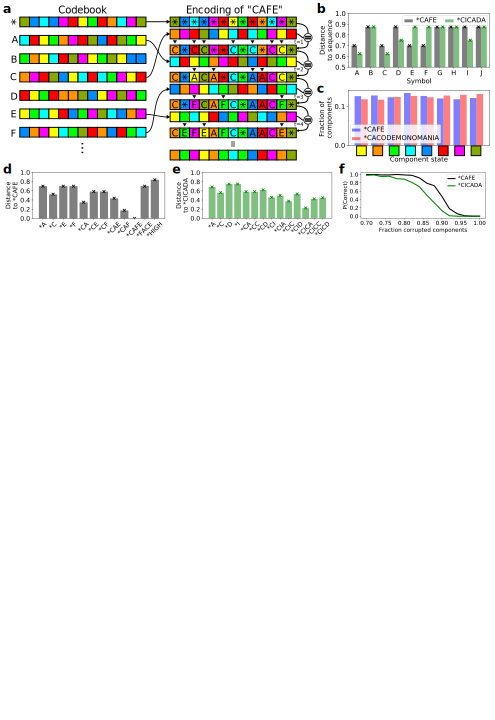
\includegraphics{1_sequences.pdf}
  \caption{Sequence encoding via crossover ($N=1024, Z=8, M=26, \gamma=1$). (a) Example encoding of CAFE; colors are states, inscribed symbols are visual aids, not used by the algorithm. (b) Sequence-symbol code distances. (c) State distributions for example short and long sequence for one $C, \mu$ sample. (d, e) Distances of CAFE's and CICADA's code to other sequence codes. (f) Decoding vs code corruption. "x"s indicate theoretical predictions and bars average simulation results. All plots here and elsewhere were made via 100 samples of $C, \mu$. "*" prefixes indicate sequences.}
  \label{fig:1}
\end{figure}

For $\gamma = 1$, $d(X^Y, X^i) \sim \textrm{Binomial}(N, 1-q)/N$, with $q = P(x^Y_j = x^i_j) = n^i/(L+1) + (1/Z)(L+1-n^i)/(L+1)$; $n^i$ is how often $i$ appears in $Y$. I.e. for large $Z$, mean symbol-sequence similarity (over $C, \mu$) scales with the symbol's count within the sequence (Fig 1b), with variance $\sim 1/N$. As exemplified by Fig 1c, crossover code components are uniform over $G$, i.i.d. for a given $Y$, and invariant to sequence statistics (e.g. length). The proof follows from the i.i.d. nature of $C, \mu$ and the interchangeability of component states, and suggests crossover as a robust, scale-invariant encoding.

For two sequences $Y$ and $Y'$ sharing their first $t$ symbols, $d(X^Y, X^{Y'})$ is also a scaled Binomial variable, and $q$ can be computed exactly for arbitrary $\gamma$; we present the $\gamma = 1$ case here. Let $\mathbf{n}_u$ be the length-$M$ symbol count vector for $Y_{1:t} = Y'_{1:t}$ with $\mathbf{1}^T\mathbf{n}_u = t$, and $\mathbf{n}_v$ and $\mathbf{n}_{v'}$ be the symbol count vectors for $Y_{t+1:L}$ and $Y'_{t+1:L'}$, respectively, with $\mathbf{1}^T\mathbf{n}_{v} = L - t$ and $\mathbf{1}^T\mathbf{n}_{v'} = L' - t$. Then:
$$q \equiv P(x_j^Y = x_j^{Y'}) = \frac{t+1}{L+1}\frac{t+1}{L'+1} + \frac{1}{L+1}\frac{1}{L'+1}\left[\mathbf{n}^T_v\mathbf{n}_{v'} + \left((L-t)(L'-t) - \mathbf{n}^T_v\mathbf{n}_{v'} \right)\frac{1}{Z}\right]$$
$$+\frac{1}{L+1}\frac{1}{L'+1}\left[
\mathbf{n}^T_{u}\mathbf{n}_{v'} + \left((t+1)(L'-t) - \mathbf{n}^T_{u}\mathbf{n}_{v'} \right)\frac{1}{Z}
+ \mathbf{n}^T_{v}\mathbf{n}_{u} + \left((L-t)(t+1) - \mathbf{n}^T_{v}\mathbf{n}_{u} \right)\frac{1}{Z}
\right]$$
For most $Y$, $X^Y$ overlaps little with $Y$'s anagrams, and more with correct than incorrect starting subsequences, e.g. codes for CI and CIC are closer to CICADA's code than codes for CD and CIA, respectively (Fig 1d,e). This is because different next-symbol candidates yield different $\mu$, which quickly decreases overlap with $X^Y$ for sequence codes with out-of-order symbols. Consequently, $Y$ can greedily decoded by rebuilding $X^Y$ from $X^*$, outputting at each rebuild step the symbol maximizing overlap with $X^Y$ when woven into the current code, then weaving it in. Of note, decoding as such is noise-robust, and when multiple $Y$ are given via a prior $P(Y)$, the mutual information between $x_j^Y$ and $Y$ is i.i.d. across $j$, yielding equivalent robustness to random and targeted attack, so decoding accuracy depends only on the number of corrupted components (Fig 1f).

For $Y$ with many symbol repeats distinct from $y_1$ (e.g. REFEREE), $X^*$ crossed over with $X^{y_1}$ can be further from $X^Y$ than $X^*$ crossed with the repeated symbol, impairing decoding. Making $\gamma > 1$, however, fixes this by more heavily weighting early symbols (Fig 2a). Surprisingly, although this front-loaded weighting improves decoding of, say, ABBBBBB, it does not equivalently degrade decoding of AAAAAAB, and optimal $\gamma$ are shared across many sequences (Fig 2b). In general, decoding accuracy decreases with L and increases with N, as the variance of $P(x_j^Y = x_j^Y')$, with $Y'$ a starting subsequence of $Y$ scales as $1/N$. Notably, decoding accuracy depends little of $M$, the dictionary size, due to the large expected distances between HD random vectors.

\begin{figure}
\label{fig:2}
  \centering
  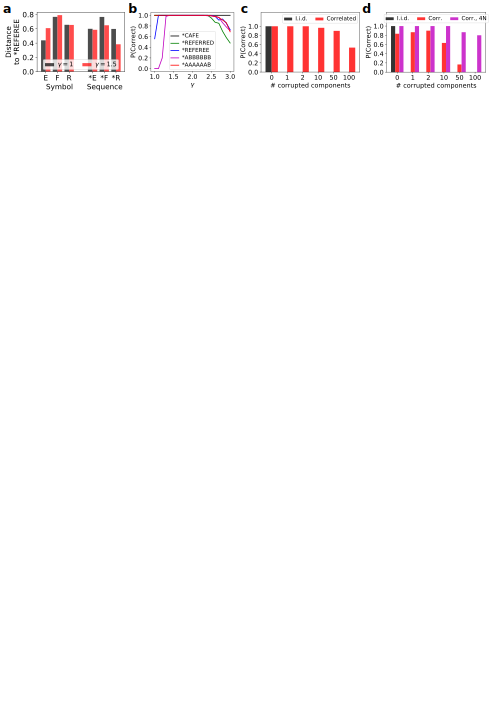
\includegraphics{2_gamma.pdf}
  \caption{Crossover modifications ($N=1024, Z=8, M=26$). (a) Distance of *REFEREE to symbols/sequences for two $\gamma$. (b) Decoding vs. $\gamma$ for several sequences. (c) Decoding of *CAFE vs number of corrupted components at encoding step for i.i.d. and correlated $\mu$. (d) Decoding of *CICADA for i.i.d., correlated $\mu$, and correlated $\mu$ with increased $N$.}
\end{figure}

While crossover with i.i.d. $\mu$ is robust to noise added to the final code (Fig 1f), it fails when noise is added during encoding (Fig 2c,d), as one altered component yields an entirely different mask. This is fixed by introducing correlations into $\mu_j(X, X')$ (here making $\mu$ a function of sparse components of $X, X'$) (Fig 2c,d). The tradeoff is decreased decoding accuracy for certain sequences, since correlated masks are less distinct, but this can be corrected via increased $N$.

Beyond sequences, crossover naturally generalizes to nested structures, or trees. Key to encoding trees is \textit{binding} elements together into groups that can themselves be bound, yet without forgetting initial group identities, e.g. ((A,B), (C,D)) must be encoded differently from ((A,D), (C,B)). In crossover, $k$ elements $i_0, ..., i_k$ can be bound into a group by using a context-dependent mask function $\mu(X^{i_0}, .... X^{i_k})$ (which can commute if within-group order does not matter). The vector for the group takes components from $X^{i_0}$ where $0 < \mu < 1/k$, from $X^{i_1}$ where $1/k < \mu < 2/k$, etc. This vector can then be bound itself in the exact same manner (Fig 3a), allowing one to recursively encode a tree of arbitrary depth. The result is a vector overlapping more with elements within vs not in the tree, and with groups within vs not in tree, even if the latter contain same base elements (Fig 3b). Generally, a tree encoding by crossover will tend to overlap more with its included sub-trees than with alternative sub-trees of equal complexity. Similar to sequence encoding, this means that both base elements and their recursive relationships can be extracted via their overlap with the crossover code, and that decoding of the full tree can occur through a recursive, but greedy reconstruction.

\begin{figure}
\label{fig:3}
  \centering
  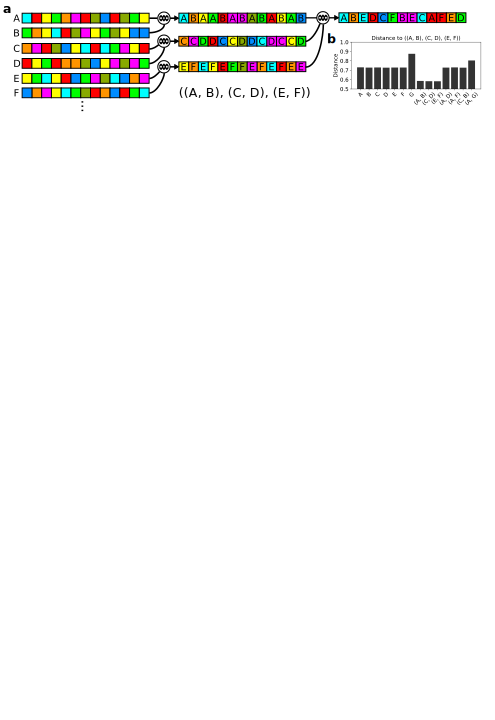
\includegraphics{3_trees.pdf}
  \caption{Tree/binding encoding via crossover ($N=1024, Z=8, M=26$). (a) Example crossover encoding of ((A,B), (C,D), (E,F)). (b) Distances of final code to element and bound-pair codes.}
\end{figure}
\section{Discussion}

While intelligent systems must learn environment statistics to operate successfully, it can useful for certain computational features to be built in \cite{Zador:2019}. Flexible compositional coding is of particular relevance as it provides a substrate for computing with novel objects/events if they are made from familiar elements: an autonomous vehicle should be able to construct and manipulate a representation of "child on scooter behind car in front of bus", even if previously it had only learned the isolated scene elements. While many trained systems, e.g. translation networks \cite{Bahdanau:2014, Luong:2015, Wu:2016}, have implicit capacity for compositional encoding (otherwise outputs would be disordered), it is unclear how they could handle complexity beyond their training data, and understanding their internal representations can be challenging \cite{Lipton:2016} (although exciting progress is being made in interpretability \cite{Zeiler:2014, Montavon:2018}). Alternatively, one can take the HDC approach of designing algorithms with \textit{a priori} flexibility, then attach or embed them in trainable systems. Basing training on convolutional binding, for instance, allowed an artificial network to learn knowledge graphs more efficiently and scalably than other methods \cite{Nickel:2016}. It stands to reason that identifying robust HDC codes could provide a useful backbone to improve artificial systems, as well as for directing our investigation of neural computation in biology.

"Crossover" shares advantages with existing HDC schemes but is distinct in key ways also. Like other schemes, crossover preserves relational information among elements, which is readily recoverable from the final code \cite{Kanerva:2009}. Further, relation codes can be reused as elements themselves, allowing arbitrary deep recursive composition \cite{Kanerva:2009}; in crossover one can add CAFE to the dictionary (perhaps with minor noise added), enabling encoding of longer sequences made from shorter ones. To encode relations, however, previous schemes have relied on circular convolution \cite{Plate:1995}, XOR (for binary vectors) \cite{Kanerva:1994}, permutation \cite{Sahlgren:2008, Gayler:1998}, or matrix multiplication \cite{Gosmann:2019}, which yields relation codes that little overlap their elements. While these distinguish different compositions of the same elements and allow cue-based recall, base elements cannot be identified directly from their overlap with the relation code, and instead require additional storage. An exception is "context-dependent thinning" (CDT), which stores relations via the union of the elements, then "stamping" the code with a context-dependent set of zeros \cite{Rachkovskij:2001}; while the stamp shape retains relational information, however, information beneath its imprint is discarded, and it is not clear how CDT could construct recursive sequence codes without early elements decaying exponentially. Crossover overcomes these limitations, as both elements and their relations can be read out directly, and in sequences no element overlaps decay exponentially. Further, crossover yields i.i.d. information across code components and code statistics invariant to object complexity, suggesting it may be a useful representation for a robust intelligent system.

Crossover is also conceptually distinct from its predecessors since one need not define arithmetical operations over code components. Whereas previous HDC algorithms require summing components, either directly or through convolution \cite{Plate:1995, Kanerva:1994, Gayler:1998, Rachkovskij:2001, Sahlgren:2008, Gosmann:2019}, crossover's component states $1, ..., Z$ are just labels, with no numeric value; they need only a comparison operation. Crossover thus outlines a distributed computation substrate that can exist outside vector spaces, and instead within more generic metric spaces. This is relevant to biological implementation, as it allows one to envision $x_j$ not only as firing rates of neurons or populations, but also as neural assembly states that might not make sense to add, multiply, or rank. For instance, each component of a crossover code could correspond to the attractor state of a 100-neuron Hopfield-like assembly \cite{Hopfield:1982}, with the collective state of a pool of $N$ such assemblies encoding a sequence or tree. Such could serve, for instance, as a crude implementation of a combinatorially expressive working memory substrate, yet with sufficient code overlap statistics to be usefully read out and manipulated by downstream and recurrent computations.

\subsubsection*{Acknowledgments}

Use unnumbered third level headings for the acknowledgments. All acknowledgments
go at the end of the paper. Do not include acknowledgments in the anonymized
submission, only in the final paper.

\bibliographystyle{unsrt}  
\bibliography{references}  %%% Remove comment to use the external .bib file (using bibtex).


%%% and comment out the ``thebibliography'' section.

% \section*{References}

% References follow the acknowledgments. Use unnumbered first-level heading for
% the references. Any choice of citation style is acceptable as long as you are
% consistent. It is permissible to reduce the font size to \verb+small+ (9 point)
% when listing the references. {\bf Remember that you can use more than eight
%   pages as long as the additional pages contain \emph{only} cited references.}
% \medskip

% \small

% [1] Alexander, J.A.\ \& Mozer, M.C.\ (1995) Template-based algorithms for
% connectionist rule extraction. In G.\ Tesauro, D.S.\ Touretzky and T.K.\ Leen
% (eds.), {\it Advances in Neural Information Processing Systems 7},
% pp.\ 609--616. Cambridge, MA: MIT Press.

% [2] Bower, J.M.\ \& Beeman, D.\ (1995) {\it The Book of GENESIS: Exploring
%   Realistic Neural Models with the GEneral NEural SImulation System.}  New York:
% TELOS/Springer--Verlag.

% [3] Hasselmo, M.E., Schnell, E.\ \& Barkai, E.\ (1995) Dynamics of learning and
% recall at excitatory recurrent synapses and cholinergic modulation in rat
% hippocampal region CA3. {\it Journal of Neuroscience} {\bf 15}(7):5249-5262.

\end{document}
